% !TeX root = ../../main.tex
\subsection{刮板刮削力学仿真}
\label{subsec:scraper_fem_sim}

“四合一”工具由刮板与毛刷两种清洁单元共同完成垢层的机械破坏：刮板依靠菱形齿的切削作用刮除垢体，毛刷依靠刷丝的刮擦、研磨与抛光作用清除残余软垢。两种单元都是通过与垢体接触过程中产生的机械力对垢体产生破坏作用的，其清洁能力的上限取决于接触应力与切削力能否超过垢体的破坏强度。为此，本节分别建立刮板刮削与刷丝受力的有限元模型，从力学角度分析两类清洁单元的作用机制，并明确刮板预紧弹簧驱动力与毛刷弹簧刚度的设计要求。

\subsubsection{刮板刮削有限元模型}
\label{subsubsec:scraper_fem_model}

（1）有限元分析模型建立

刮板的结构虽然复杂，但其与井筒管壁的作用区域局限在刮板齿部，齿形以外的部位并不直接参与除垢。刮板对钡锶垢的挤压变形与刮削过程涉及接触状态的反复变化以及垢体的屈服与破裂，属于高度非线性问题，按三维模型计算需要占用大量计算资源。为此，将三维问题简化为二维平面问题，这样处理不仅可以大幅提高运算速度，对计算结果的影响也较小。简化后的有限元计算模型如图\ref{fig:scraper_fem_model}所示，模型由套管壁、钡锶垢层与刮板齿三部分组成，套管壁与钡锶垢相贴合，刮板齿顶与垢层接触。

\begin{figure}[htbp]
	\centering
	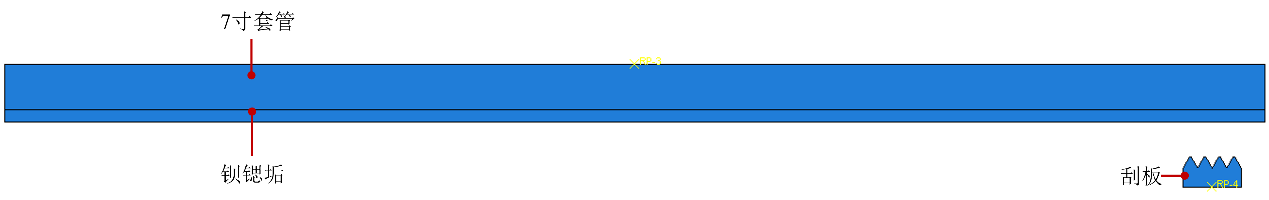
\includegraphics[width=\textwidth]{figure/chapter3/4in1-sim/scraper-fem-model.png}
	\caption{刮板刮削简化力学模型}
	\label{fig:scraper_fem_model}
\end{figure}

（2）接触定义

模型中各构件之间存在接触关系，需要考虑摩擦，因此需对发生接触行为的构件定义摩擦因数。分析中采用通用接触，切向行为采用罚函数的摩擦公式，法向行为采用硬接触，摩擦系数取0.15。

（3）约束与载荷施加

仿真设置两个分析步：第一步模拟刮板在弹簧驱动力作用下完成与钡锶垢的挤压接触，此过程中对套管及钡锶垢施加固定约束；第二步模拟刮板在驱动位移作用下移动，完成对钡锶垢的刮削。约束与载荷的施加位置如图\ref{fig:scraper_boundary}所示。

\begin{figure}[htbp]
	\centering
	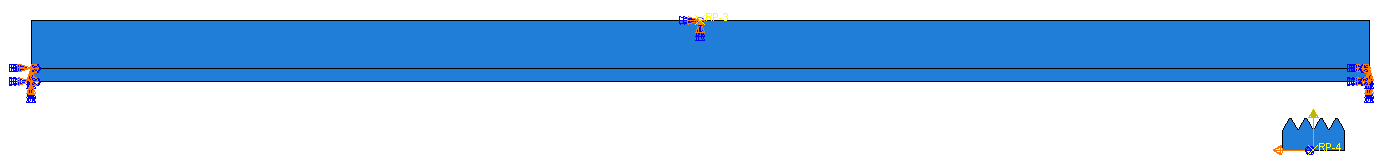
\includegraphics[width=\textwidth]{figure/chapter3/4in1-sim/scraper-boundary-conditions.png}
	\caption{刮板模块组成及边界条件施加}
	\label{fig:scraper_boundary}
\end{figure}

（4）网格划分

刮板与钡锶垢的接触及刮削过程是本节的主要研究内容，为获得更准确的结果，应对刮板齿及钡锶垢进行网格加密。但网格并非越密越好：网格较粗时，提高网格密度可使计算精度显著提高；当网格数量增加到一定程度后，继续提高网格密度对精度的改善很小，反而成倍增加计算时间、降低求解效率。因此，在对刮板及钡锶垢划分网格前，需先进行网格无关性验证。

计算采用CPS4R四节点双线性平面应力四边形单元，网格尺寸分别取3.0、2.5、2.0、1.5、1.0和0.8\,mm，计算得到的最大应力分别为146.7、160.3、173.8、181.4、185.6和186.1\,MPa，见表\ref{tab:mesh_independence}与图\ref{fig:mesh_independence}。由表可见，网格尺寸由1.0\,mm加密至0.8\,mm时，最大应力仅变化0.3\%，远小于3\%的精度要求，说明网格尺寸为1.0\,mm时已达到精度要求；而继续加密将使计算时间成倍增加，大幅降低求解效率。故本研究选用1.0\,mm的网格开展刮削仿真分析，同时将刮板齿与钡锶垢之间的接触面进行网格加密，网格划分如图\ref{fig:scraper_mesh}所示。

\begin{table}[htbp]
	\centering
	\caption{网格无关性验证结果}
	\label{tab:mesh_independence}
	\renewcommand{\arraystretch}{1.3}
	\begin{tabularx}{0.7\textwidth}{CC}
		\toprule
		\textbf{网格尺寸/mm} & \textbf{最大应力/MPa} \\
		\midrule
		3.0 & 146.7 \\
		2.5 & 160.3 \\
		2.0 & 173.8 \\
		1.5 & 181.4 \\
		1.0 & 185.6 \\
		0.8 & 186.1 \\
		\bottomrule
	\end{tabularx}
\end{table}

\begin{figure}[htbp]
	\centering
	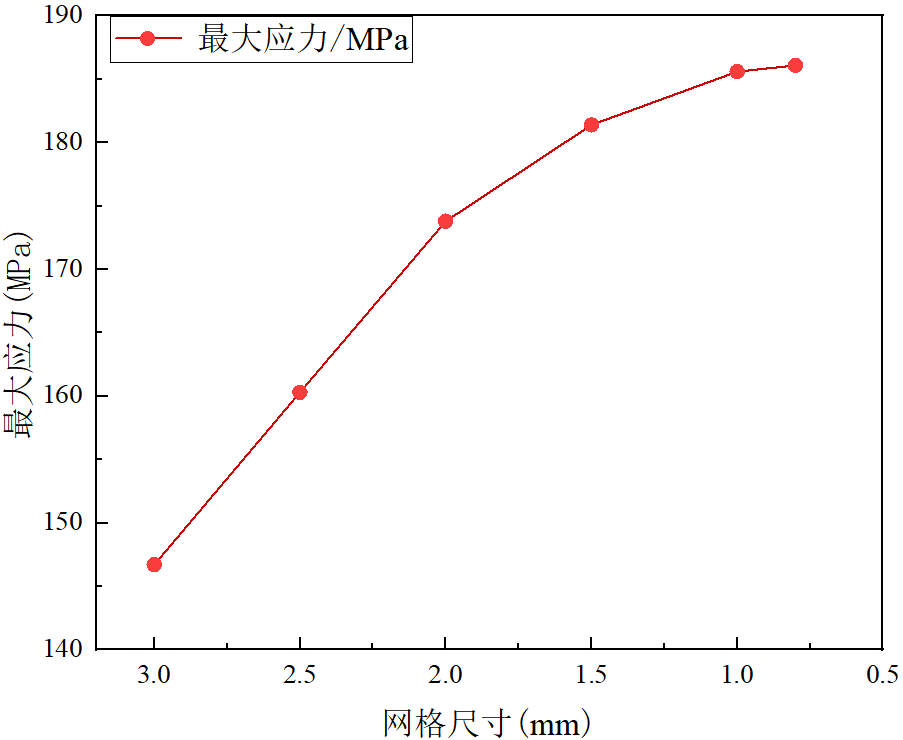
\includegraphics[width=0.55\textwidth]{figure/chapter3/4in1-sim/mesh-independence.png}
	\caption{网格无关性验证}
	\label{fig:mesh_independence}
\end{figure}

\begin{figure}[htbp]
	\centering
	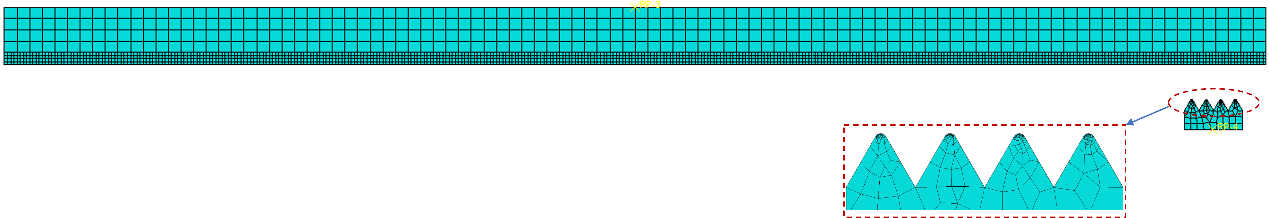
\includegraphics[width=\textwidth]{figure/chapter3/4in1-sim/scraper-mesh.png}
	\caption{刮板及钡锶垢的网格划分}
	\label{fig:scraper_mesh}
\end{figure}

\subsubsection{弹簧驱动力对刮削效果的影响}
\label{subsubsec:driving_force_effect}

弹簧驱动力是刮板能否有效除垢的决定性因素：驱动力过小时刮板齿难以压入并切透垢层，过大时又会因齿面被细屑充填、浮动支撑压死而使刮削能力下降。为确定合理的设计值，分别对刮板底部施加150、180、250和300\,N的弹簧驱动力进行刮削仿真，统计刮削过程中的平均切削力，并观察垢层的残留情况，结果汇总于表\ref{tab:driving_force}。

当刮板底部施加150\,N弹簧驱动力时，刮削效果未能达到预期（图\ref{fig:scraping_effect}(a)）。该工况下刮板对钡锶垢的清除作用十分有限，基本无法实现有效刮削；刮削过程中的平均作用力仅为202.87\,N（图\ref{fig:cutting_force}(a)），明显不足以克服钡锶垢与基体之间的结合力，从而导致刮削失败。这一结果验证了150\,N的弹簧驱动力无法满足钡锶垢清除的基本要求。

当弹簧驱动力提高至180\,N时，刮削结果（图\ref{fig:scraping_effect}(b)）显示，相较于150\,N工况，刮板对钡锶垢的清除效果有所改善，但仍存在明显的垢层残留问题。该工况下刮板与钡锶垢之间的平均切削力达到230.46\,N（图\ref{fig:cutting_force}(b)），较150\,N工况提高了13.6\%，仍未能完全克服垢层与基体的结合强度，导致刮削不彻底。这一结果表明，180\,N的弹簧驱动力虽能部分提升刮削性能，但仍需进一步提高驱动力才能获得更理想的除垢效果。

在150\,N与180\,N驱动力均未能有效清除钡锶垢的情况下，将弹簧驱动力增大至250\,N进行仿真（图\ref{fig:scraping_effect}(c)）。该工况下刮削性能显著改善：一方面，平均切削力提升至389.15\,N（图\ref{fig:cutting_force}(c)），较180\,N工况增幅达68.8\%；另一方面，刮板能够较好地完成钡锶垢的主要刮削作业。然而，通过表面形貌观察发现，刮削区域仍存在局部钡锶垢残留现象，说明该驱动力水平虽已接近、但尚未完全达到彻底清除垢层所需的临界值，为进一步确定临界驱动力提供了依据。

为进一步提升刮削效果，在250\,N驱动力下仍存在残留的情况下，将弹簧驱动力提升至300\,N进行仿真验证（图\ref{fig:scraping_effect}(d)）。该工况下刮削性能实现突破性提升：平均切削力达到473.56\,N（图\ref{fig:cutting_force}(d)），较250\,N工况提升约35\%。仿真结果表明，300\,N的驱动力完全满足钡锶垢清除需求，刮板能够彻底清除表面垢层，无残留现象。

\begin{table}[H]
	\centering
	\caption{不同弹簧驱动力下的刮削仿真结果}
	\label{tab:driving_force}
	\renewcommand{\arraystretch}{1.3}
	\begin{tabularx}{\textwidth}{ccc>{\raggedright\arraybackslash}X}
		\toprule
		弹簧驱动力/N & 平均切削力/N & 较前一工况增幅/\%} & 垢层清除效果 \\
		\midrule
		150 & 202.87 & — & 基本无法实现有效刮削 \\
		180 & 230.46 & 13.6 & 有所改善，仍存在明显残留 \\
		250 & 389.15 & 68.8 & 主要垢层被刮除，局部残留 \\
		300 & 473.56 & 35.0 & 完全清除，无残留 \\
		\bottomrule
	\end{tabularx}
\end{table}

\begin{figure}[htbp]
	\centering
	\subfloat[150\,N]{%
	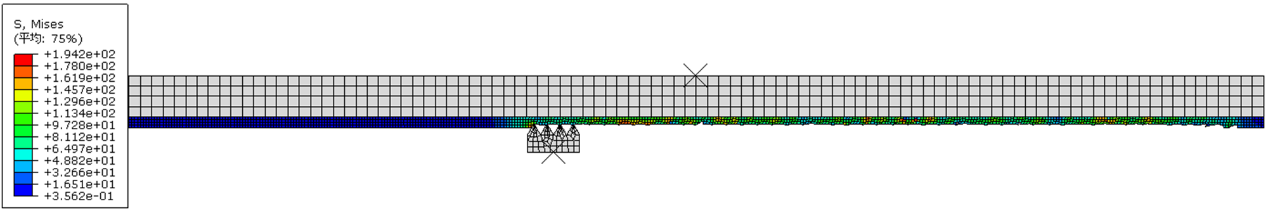
\includegraphics[width=\textwidth]{figure/chapter3/4in1-sim/scraping-effect-150n.png}
	}
	\vspace{0.5em}
	\subfloat[180\,N]{%
	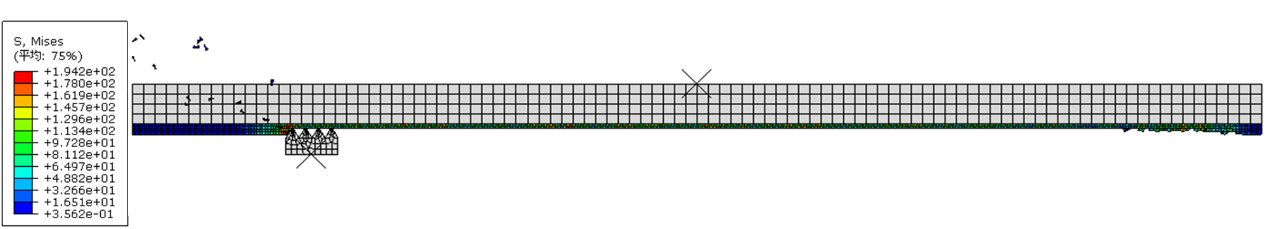
\includegraphics[width=\textwidth]{figure/chapter3/4in1-sim/scraping-effect-180n.png}
	}
	\vspace{0.5em}
	\subfloat[250\,N]{%
	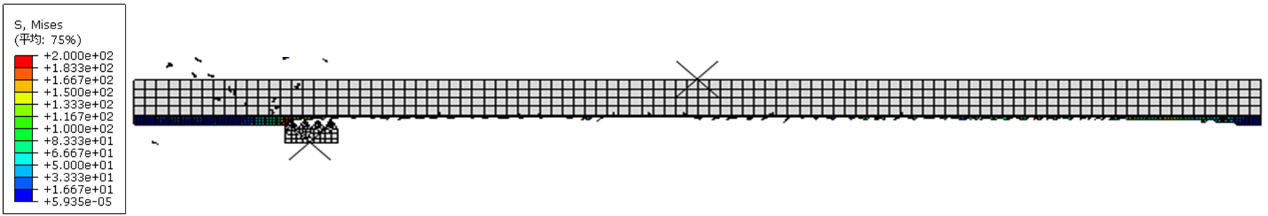
\includegraphics[width=\textwidth]{figure/chapter3/4in1-sim/scraping-effect-250n.png}
	}
	\vspace{0.5em}
	\subfloat[300\,N]{%
	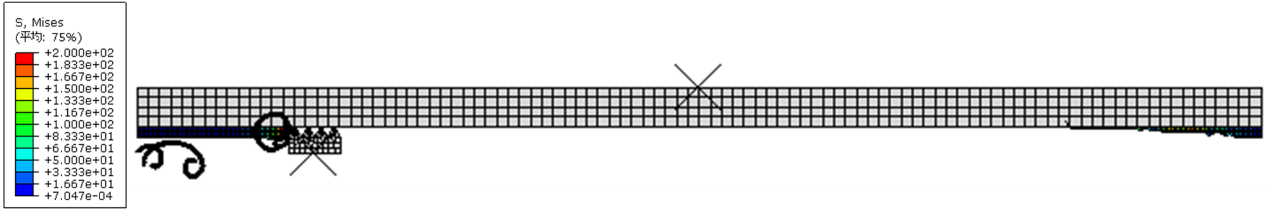
\includegraphics[width=\textwidth]{figure/chapter3/4in1-sim/scraping-effect-300n.png}
	}
	\caption{不同弹簧驱动力作用下的刮削效果}
	\label{fig:scraping_effect}
\end{figure}

\begin{figure}[htbp]
	\centering
	\subfloat[150\,N]{%
	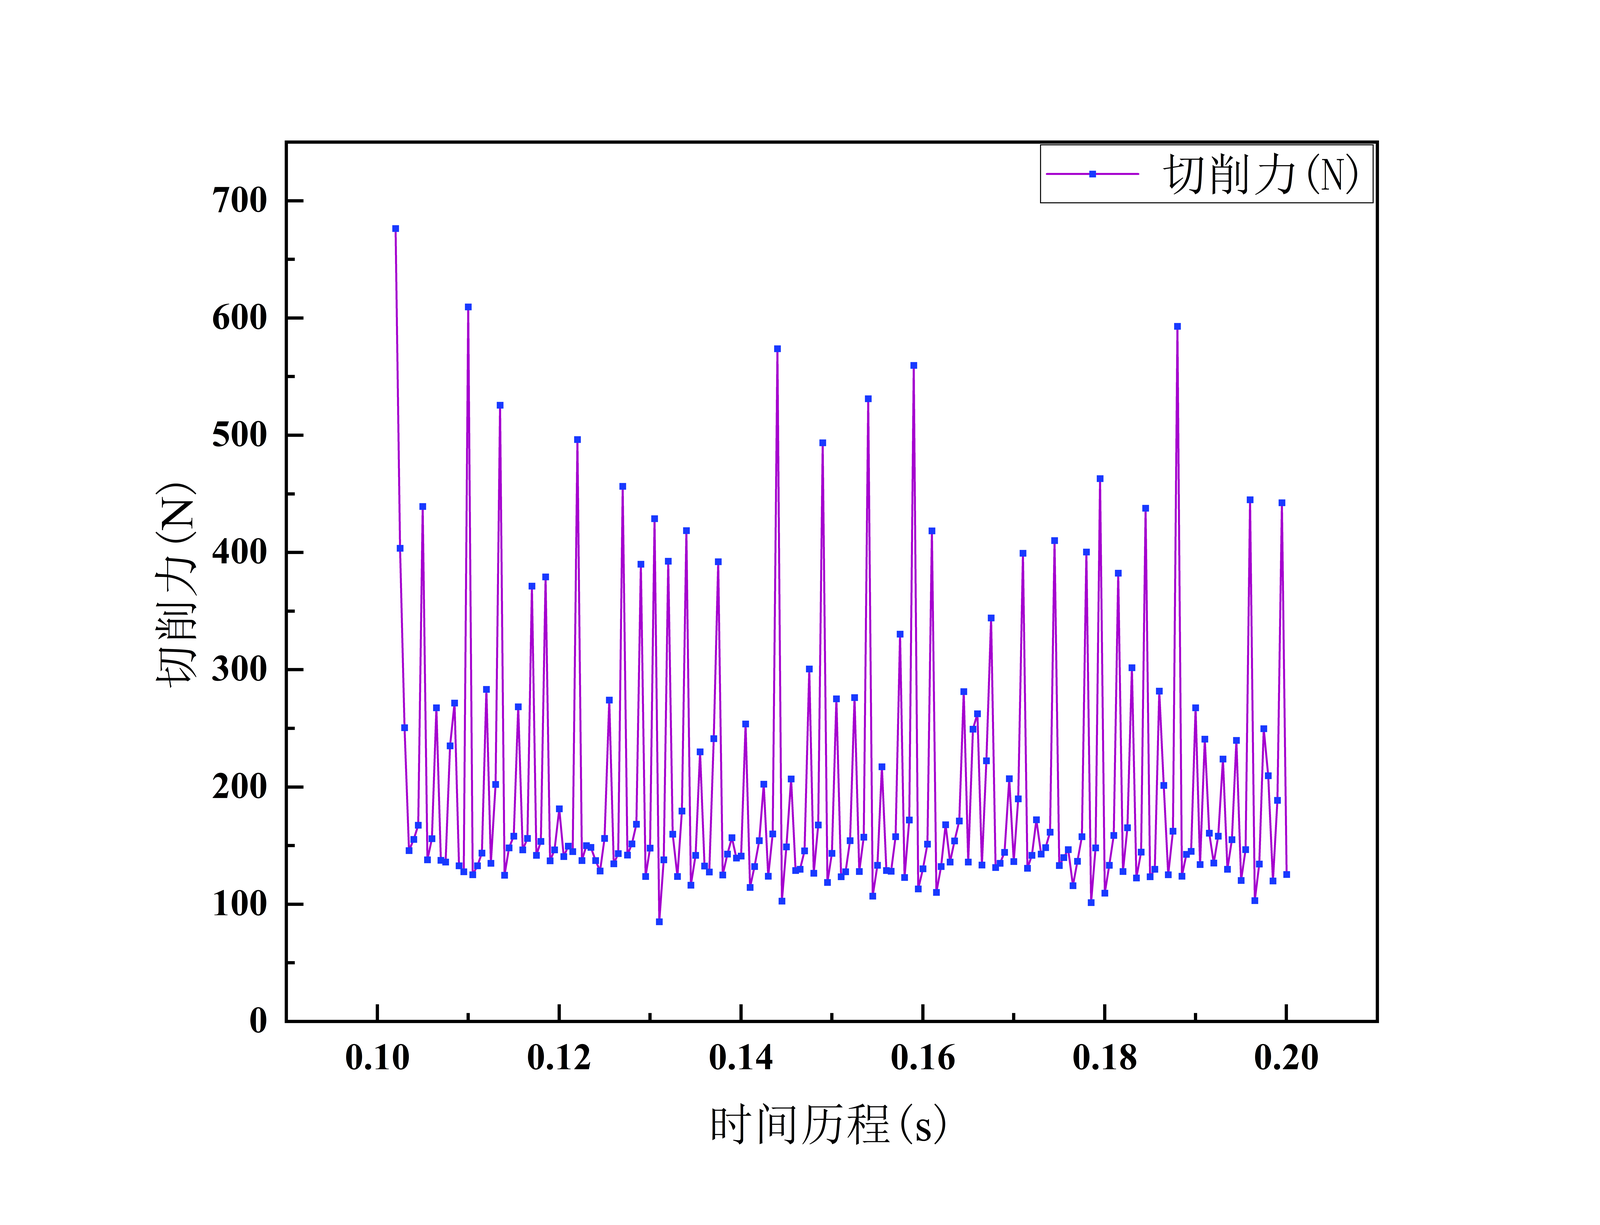
\includegraphics[width=0.47\textwidth]{figure/chapter3/4in1-sim/cutting-force-150n.png}
	}
	\hfill
	\subfloat[180\,N]{%
	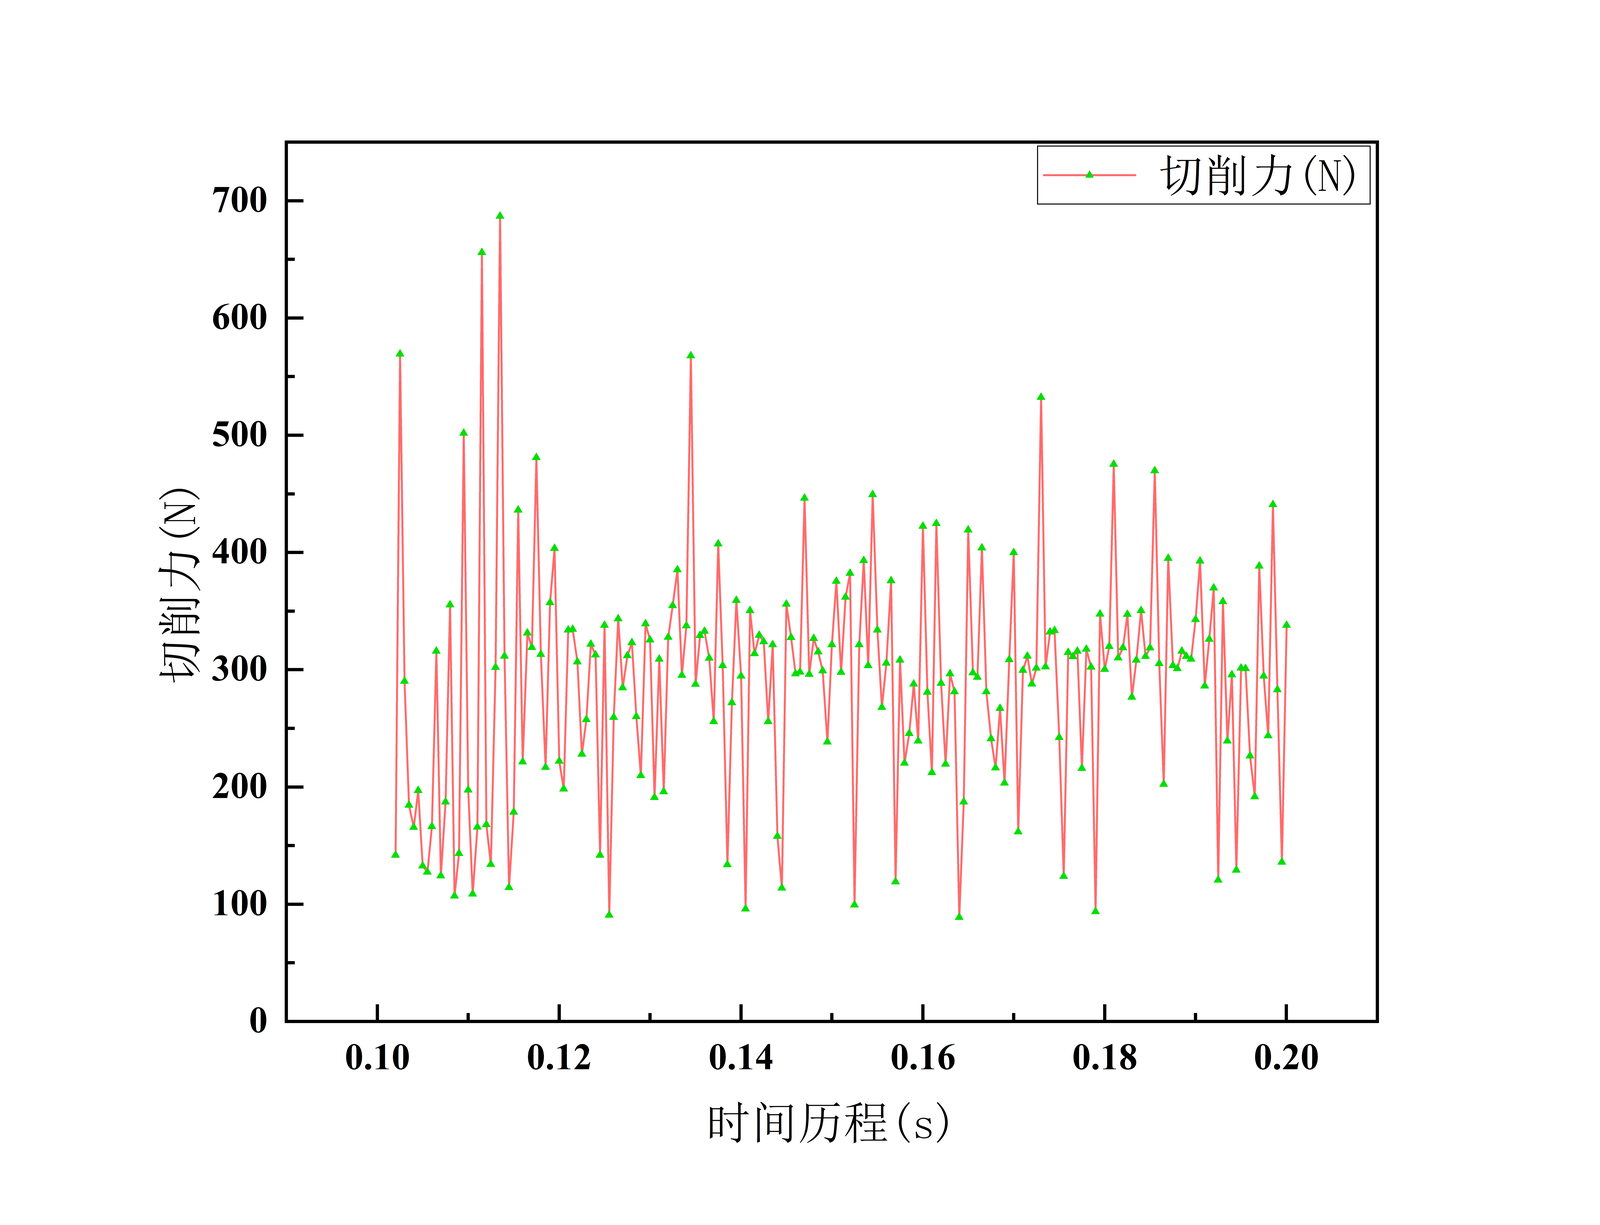
\includegraphics[width=0.47\textwidth]{figure/chapter3/4in1-sim/cutting-force-180n.png}
	}
	\\[1em]
	\subfloat[250\,N]{%
	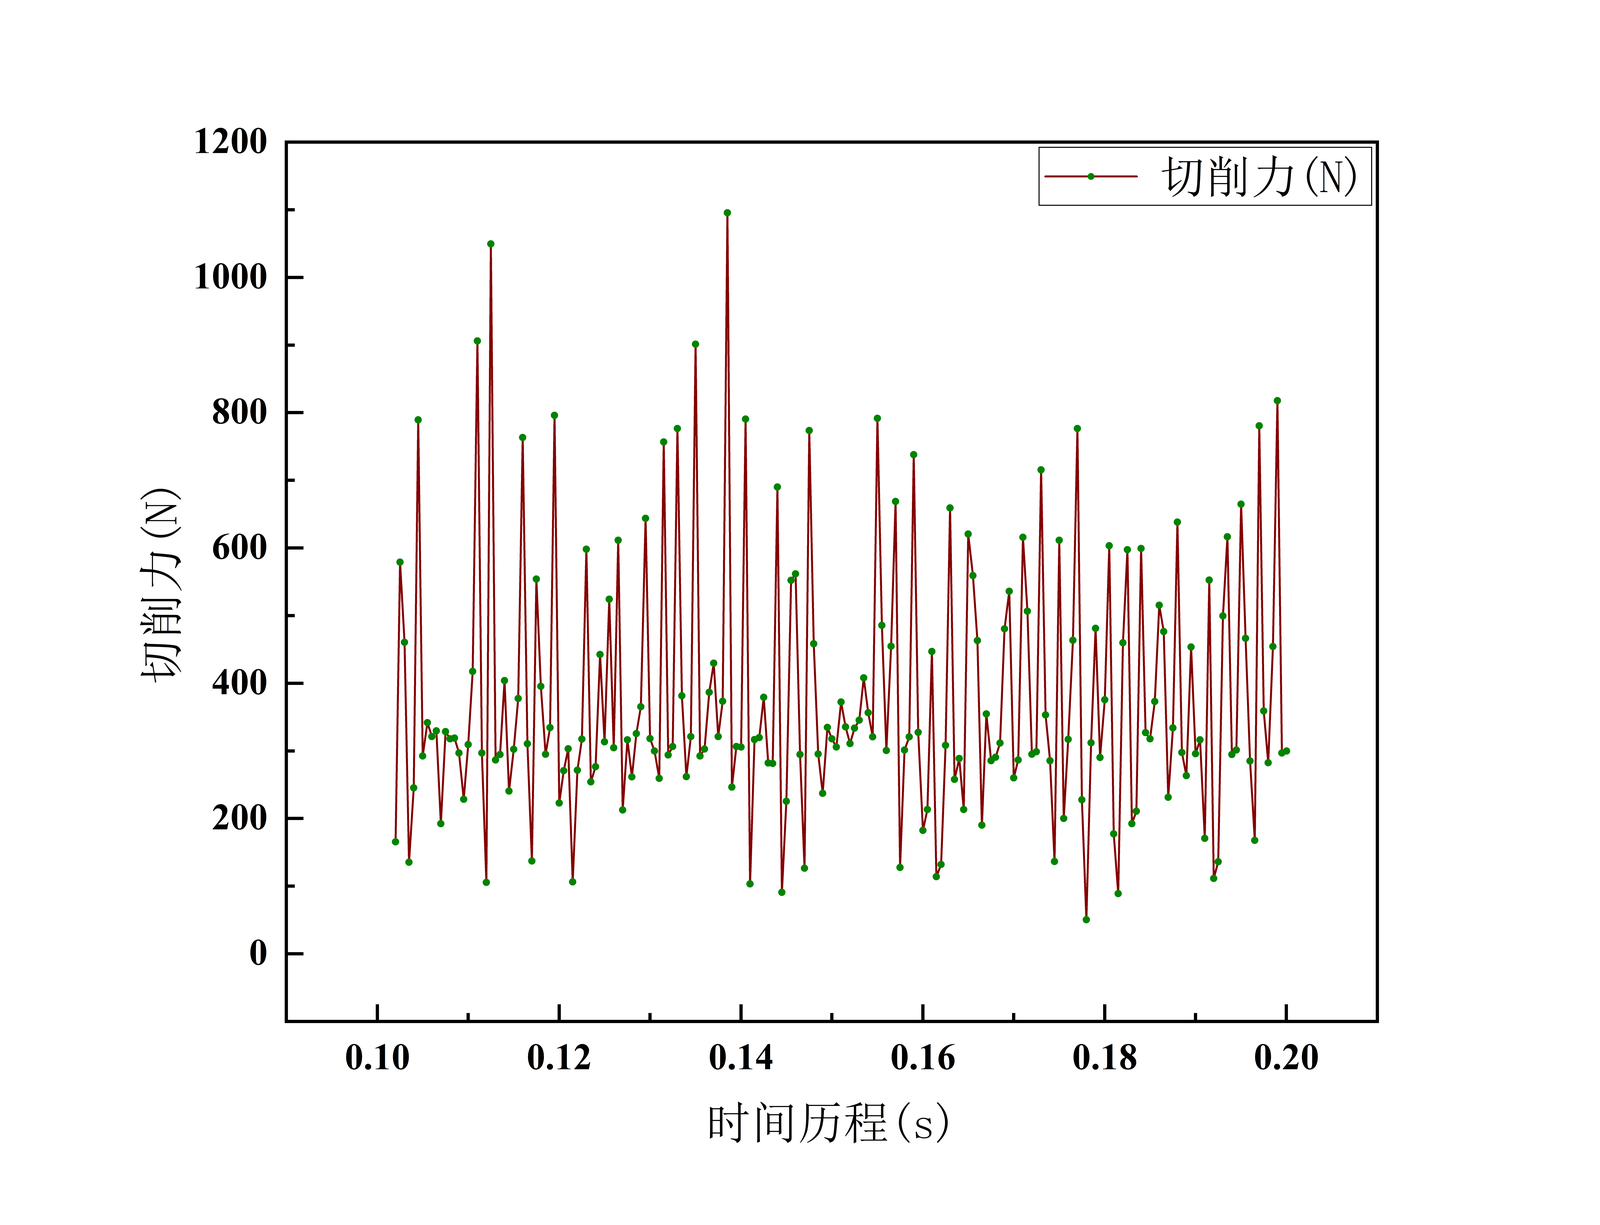
\includegraphics[width=0.47\textwidth]{figure/chapter3/4in1-sim/cutting-force-250n.png}
	}
	\hfill
	\subfloat[300\,N]{%
	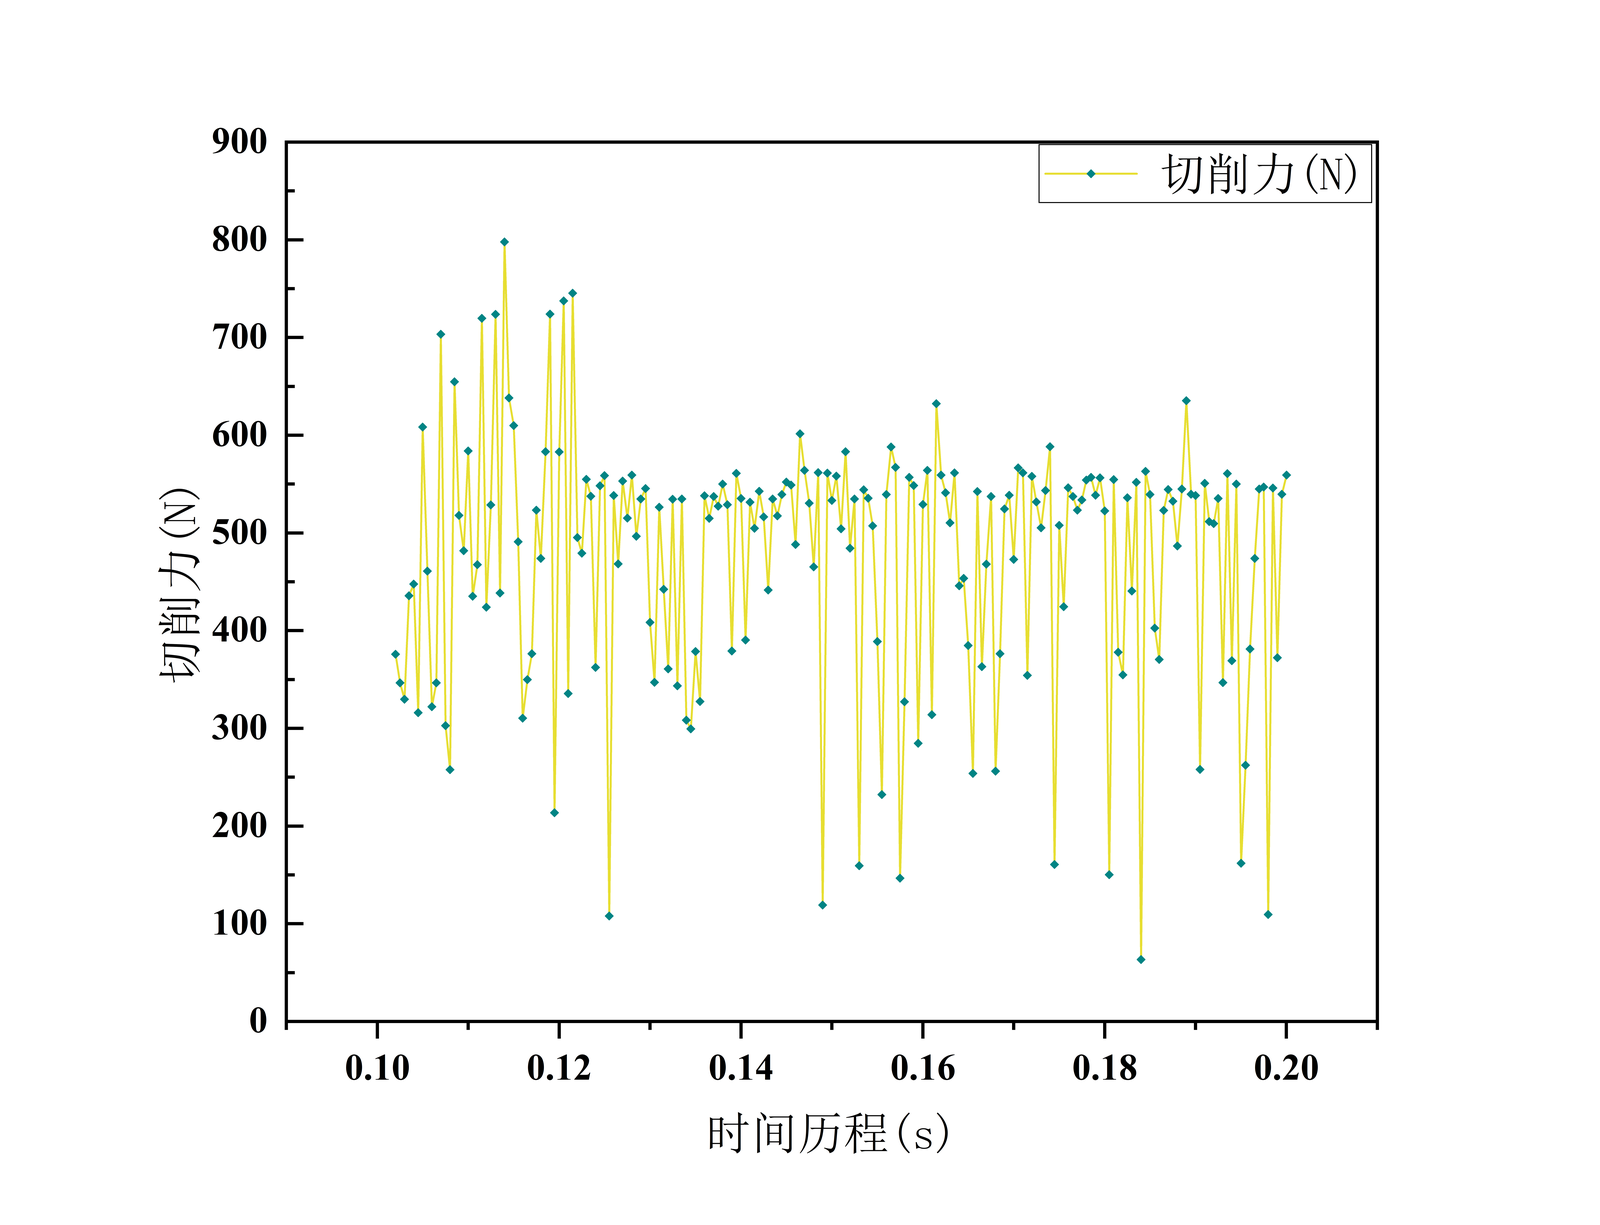
\includegraphics[width=0.47\textwidth]{figure/chapter3/4in1-sim/cutting-force-300n.png}
	}
	\caption{不同弹簧驱动力作用下的刮板切削力}
	\label{fig:cutting_force}
\end{figure}

通过对不同弹簧驱动力作用下的刮削效果开展仿真分析，得到如下结果。

\begin{enumerate}[label=（\arabic*）,leftmargin=2.6em,itemsep=2pt]
\item \textbf{临界驱动力阈值。}当弹簧驱动力达到300\,N时，平均切削力提升至473.56\,N，可实现垢层的完全清除且无残留现象，可将该值作为刮板预紧弹簧驱动力的设计下限。

\item \textbf{驱动力与清除效果的相关性。}驱动力与清除效果呈非线性正相关：驱动力由150\,N提高至300\,N的过程中，平均切削力增幅达133\%，清除效果实现从“基本无效”到“完全清除”的质变。其原因是，在切削力尚未超过垢体与基体的结合强度之前，刮板齿主要沿垢面挤压、摩擦滑移，切除量很小；只有当驱动力使切削力足以克服结合强度时，垢层才会以脆性破碎的方式成片剥落。

\item \textbf{工程应用指导价值。}150$\sim$250\,N的中等驱动力区间虽能实现部分清除，但存在明显残留；300\,N及以上的驱动力可保证除垢的彻底性与工程应用的可靠性。需要说明的是，上述驱动力为二维模型中施加的数值，用于比较不同工况下的刮削效果，实际弹簧预紧力的确定还应结合前述弹簧的力学计算，按弹簧刚度与压缩行程进行换算，并使弹簧压缩量不超过刮板浮动支撑的径向行程。
\end{enumerate}

\subsection{毛刷力学仿真}
\label{subsec:brush_fem_sim}

“四合一”工具的毛刷模块安装于刮刀模块之后，用于清除刮削后残留的细小垢屑。目前对毛刷的研究以实验为主，研究重点多为钢丝刷对金属表面的抛光作用，对其接触力学行为的研究相对较少。本节以单根刷丝为研究对象，根据刷丝在表面弹力作用下产生弹性变形而形成的接触应力，研究其对垢体的去除效果。

毛刷结构如图\ref{fig:brush_structure}所示。刷毛的伸出长度为15\,mm，整个刷毛与套管之间的单边过盈量为5\,mm，即工具入井后刷丝需沿径向产生5\,mm的变形才能通过套管。为了保护刷丝工作的稳定性，在刷板下设弹簧支撑结构。

\begin{figure}[htbp]
	\centering
	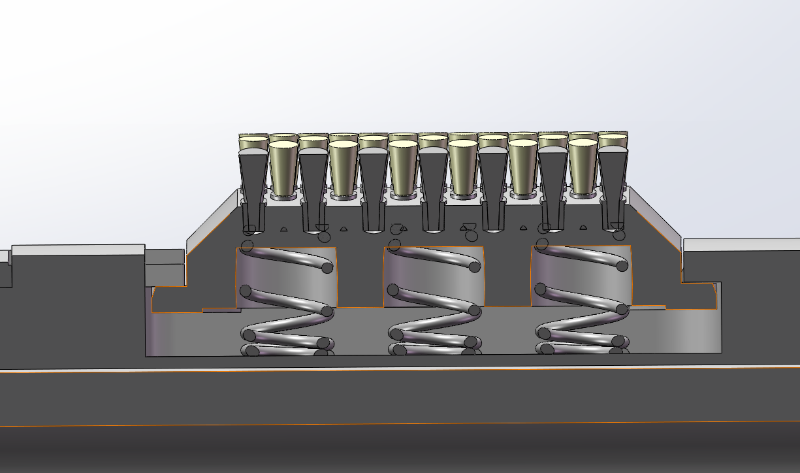
\includegraphics[width=0.72\textwidth]{figure/chapter3/4in1-sim/brush-structure.png}
	\caption{工具上毛刷结构}
	\label{fig:brush_structure}
\end{figure}

考虑到刷丝在入井过程中存在磨损，将刷丝末端处理为球头，建立的刷丝与垢体相互作用的仿真模型如图\ref{fig:brush_model}所示。井下清洁工具中钢丝刷的常用材料为304奥氏体不锈钢，选材依据主要是丝材的耐腐蚀性能；但材料、刷丝长度及其他几何参数对刷丝性能的影响同样值得研究。

\begin{figure}[htbp]
	\centering
	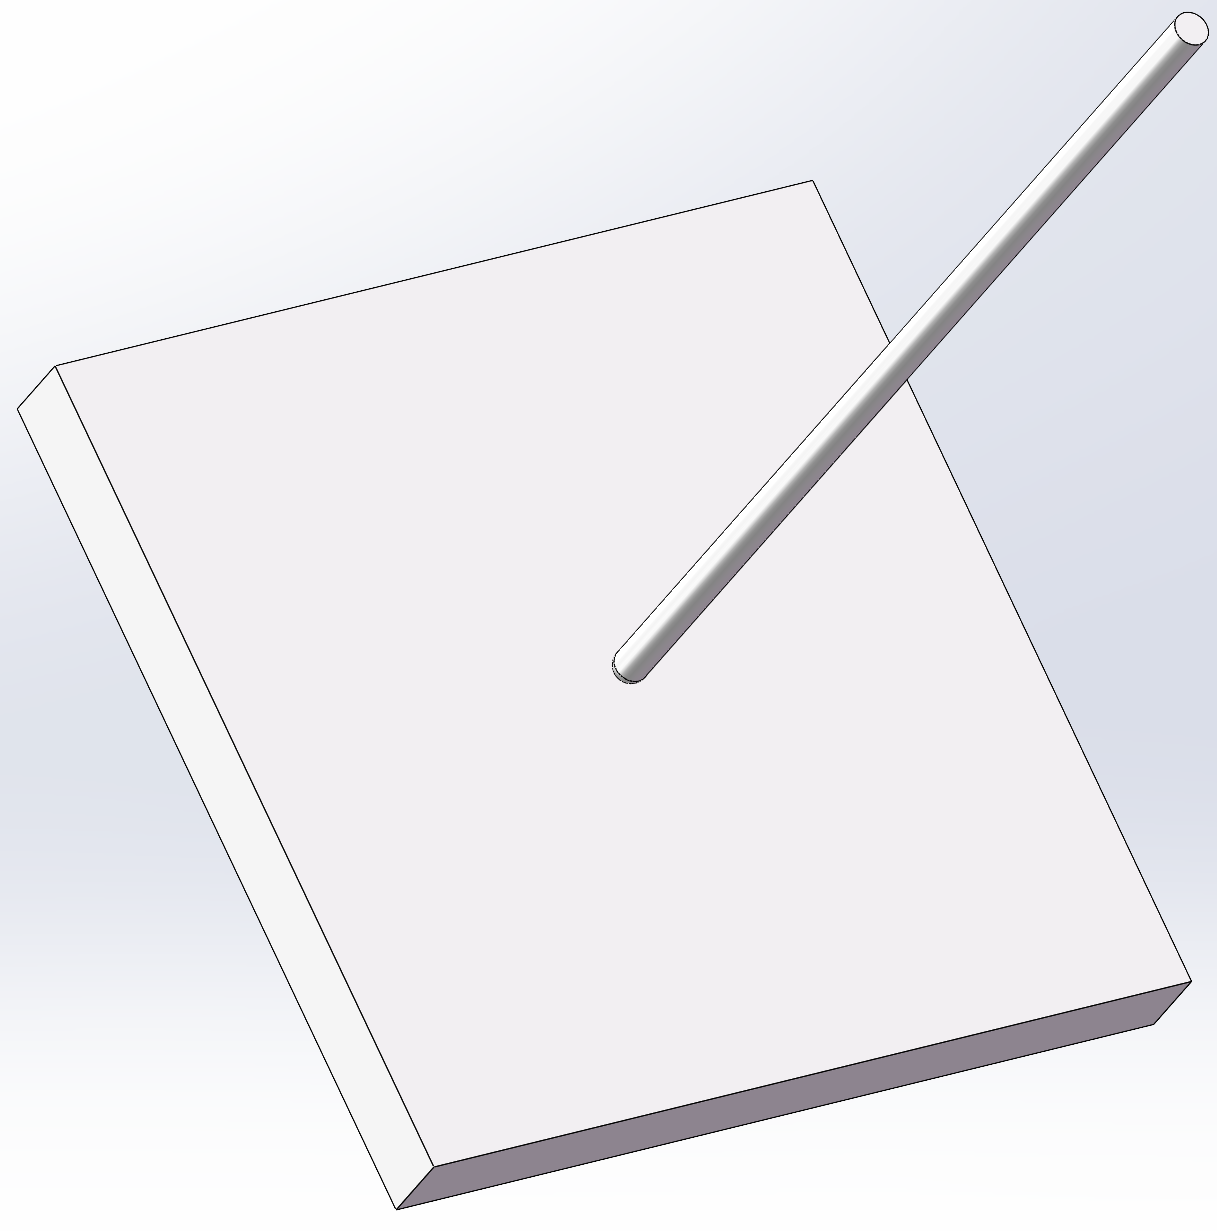
\includegraphics[width=0.42\textwidth]{figure/chapter3/4in1-sim/brush-wire-model.png}
	\caption{刷丝—垢体相互作用仿真模型}
	\label{fig:brush_model}
\end{figure}

计算取刷丝的径向位移为0.25、0.5和0.75\,mm，刷丝与垢体（或管壁）之间的接触应力变化如图\ref{fig:brush_contact_stress}与表\ref{tab:brush_contact_stress}所示。随着径向位移的增大，最大接触应力呈先略微增加、后下降的趋势：径向位移由0.25\,mm增至0.5\,mm时，最大接触应力由2.44\,MPa增至2.47\,MPa；径向位移增至0.75\,mm时，最大接触应力降至1.65\,MPa。其原因是：刷丝为长悬臂结构，当刷丝产生较大的径向变形时会发生结构屈曲，径向刚度下降，进而导致刷丝与垢体（或管壁）之间的接触力和接触应力下降。

\begin{figure}[htbp]
	\centering
	\subfloat[径向位移0.25\,mm]{%
	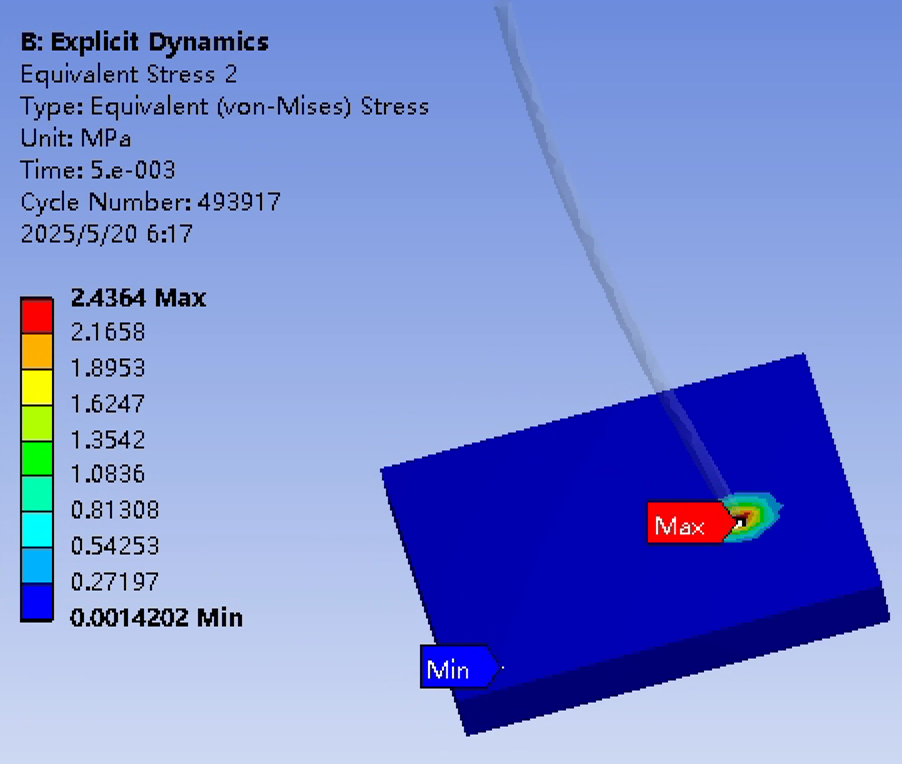
\includegraphics[width=0.32\textwidth]{figure/chapter3/4in1-sim/brush-contact-stress-1.png}
	}
	\hfill
	\subfloat[径向位移0.5\,mm]{%
	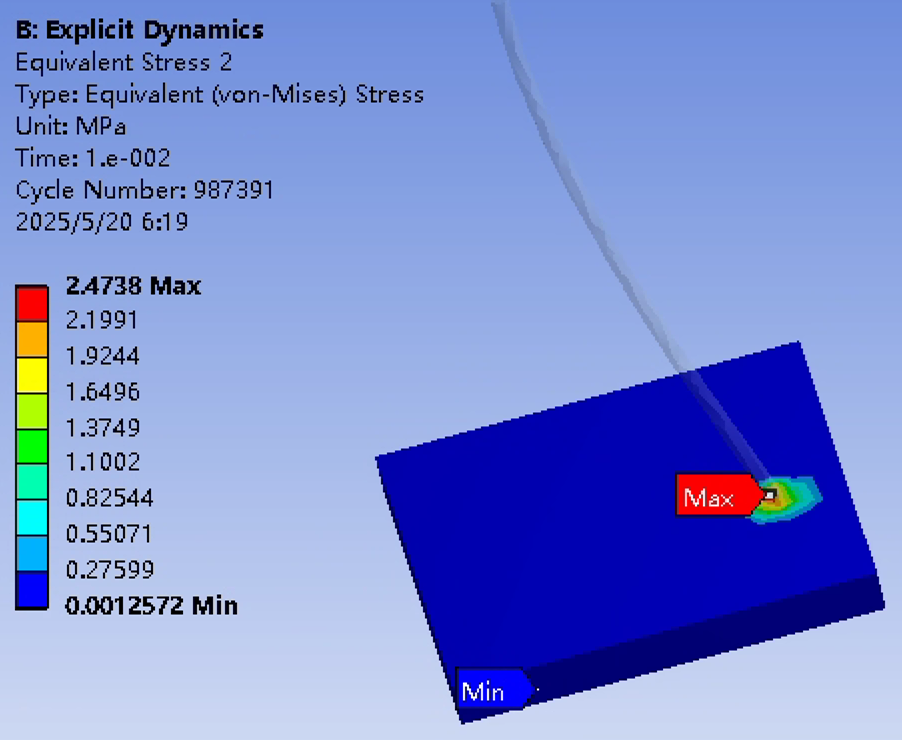
\includegraphics[width=0.32\textwidth]{figure/chapter3/4in1-sim/brush-contact-stress-2.png}
	}
	\hfill
	\subfloat[径向位移0.75\,mm]{%
	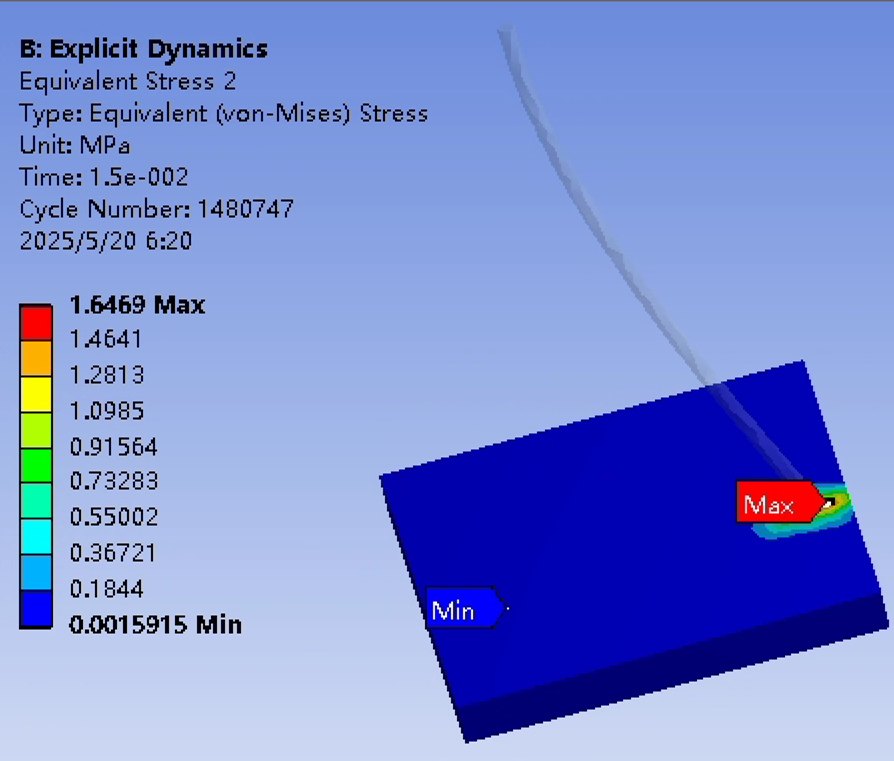
\includegraphics[width=0.32\textwidth]{figure/chapter3/4in1-sim/brush-contact-stress-3.png}
	}
	\caption{刷丝对垢体表面产生的接触应力变化情况}
	\label{fig:brush_contact_stress}
\end{figure}

\begin{table}[H]
	\centering
	\caption{不同径向位移下刷丝与垢体间的最大接触应力}
	\label{tab:brush_contact_stress}
	\renewcommand{\arraystretch}{1.3}
	\begin{tabularx}{0.85\textwidth}{cc>{\raggedright\arraybackslash}X}
		\toprule
		\textbf{径向位移/mm} & \textbf{最大接触应力/MPa} & \textbf{刷丝受力状态} \\
		\midrule
		0.25 & 2.44 & 屈曲前，刚度基本不变 \\
		0.50 & 2.47 & 接近屈曲，接触应力最高 \\
		0.75 & 1.65 & 已发生屈曲，刚度下降 \\
		\bottomrule
	\end{tabularx}
\end{table}

本算例中刷丝的长径比为37.5，对应的相对径向变形量为3.33\%。在刷丝结构发生屈曲之前，不同长径比刷丝的变形行为应具有相似性。因此，在毛刷清洁单元设计时，应合理设计刷板下弹簧的刚度，使刷丝的相对径向变形量控制在3.33\%左右，避免刷丝过早屈曲而丧失接触压力。

刷丝与垢体（或管壁）之间的接触应力在2.5\,MPa左右，该量级说明：第一，毛刷只能直接清理强度不高的软垢；第二，刷丝不能直接破坏表面平整的硬垢，其对作用表面主要起到类似刮擦与抛光的作用。因此，在去除硬质垢体时毛刷的作用较弱，不能独立使用，必须与其他清洁单元联合使用；当其他清洁单元先破坏垢体结构、形成粗糙表面后，刷丝对垢体的微小凸起可产生较强的接触应力，从而对其产生切削作用。

可以预见，通过减小刷丝长度、提高刷丝刚度的方法来提高毛刷对硬垢的清洁效果是有限的，原因是垢体的强度通常比刷丝的接触应力高一个数量级，超出了改变刷丝长度所能达到的合理范围。此外，改变刷丝材料也难以显著增强毛刷的清洁能力：对计算结果产生显著影响的材料属性是刷丝的弹性模量与泊松比，而二者的变化范围都比较小，例如大多数钢材的泊松比在0.28$\sim$0.30之间，杨氏模量在190$\sim$210\,GPa之间。毛刷的结构与材料受生产加工条件和使用要求的限制往往相对固定，本项目中毛刷的选材应主要考虑材料的防腐性能，选用304奥氏体不锈钢即可满足需求。

\subsection{刮板与毛刷清洁作用机制小结}
\label{subsec:cleaning_mechanism_summary}

综合上述刮板与毛刷的仿真结果，得到如下结论。

\begin{enumerate}[label=（\arabic*）,leftmargin=2.6em,itemsep=2pt]
\item 建立了刮板刮削的二维有限元模型，经网格无关性验证确定网格尺寸为1.0\,mm；仿真表明，弹簧驱动力与钡锶垢的清除效果呈非线性正相关，驱动力达300\,N、平均切削力473.56\,N时可将垢层完全清除，为实际工况下驱动力参数的选择提供了依据。

\item 刷丝与垢体（或管壁）之间的接触应力约为2.5\,MPa，毛刷适用于清理软垢，对硬垢的清洁效果有限，需与其他清洁单元联合使用；改变刷丝长度或材料难以显著提升其清洁能力，刷丝选材应优先考虑防腐性能，304奥氏体不锈钢可满足项目需求。
\end{enumerate}
